\documentclass{beamer}
\usepackage[utf8]{inputenc}
\usepackage[T1]{fontenc}
\usepackage[portuguese]{babel}

\usetheme{Madrid}
\usecolortheme{beaver}

\title{Comparação dos Algoritmos}
\author[Laboratório de Sistemas II]{André Costa Batista}
\institute[2025/2]{Universidade Federal de Minas Gerais\\Escola de Engenharia\\ELE634 Laboratório de Sistemas II}
\date{\today}

\begin{document}

\frame{\titlepage}

\begin{frame}
\frametitle{Sumário}
\tableofcontents
\end{frame}

\section{Considerações Iniciais}
\begin{frame}
\frametitle{Considerações Iniciais}
\begin{itemize}
    \item 30 execuções para cada algoritmo em cada instância.
    \item Apenas as soluções finais factíveis foram consideradas.
    \item Desativação no código das sementes fixas para garantir maior variabilidade entre as execuções.
    \item Conferência de contações de avaliações: tudo certo.
\end{itemize}
\end{frame}

\section{Instância Pequena}
\begin{frame}
\frametitle{Resultados}
\framesubtitle{Instância Pequena}
\begin{itemize}
    \item Apenas 1 execução do Seu Jorge resultou em solução não factível.
\end{itemize}
\begin{figure}
    \centering
    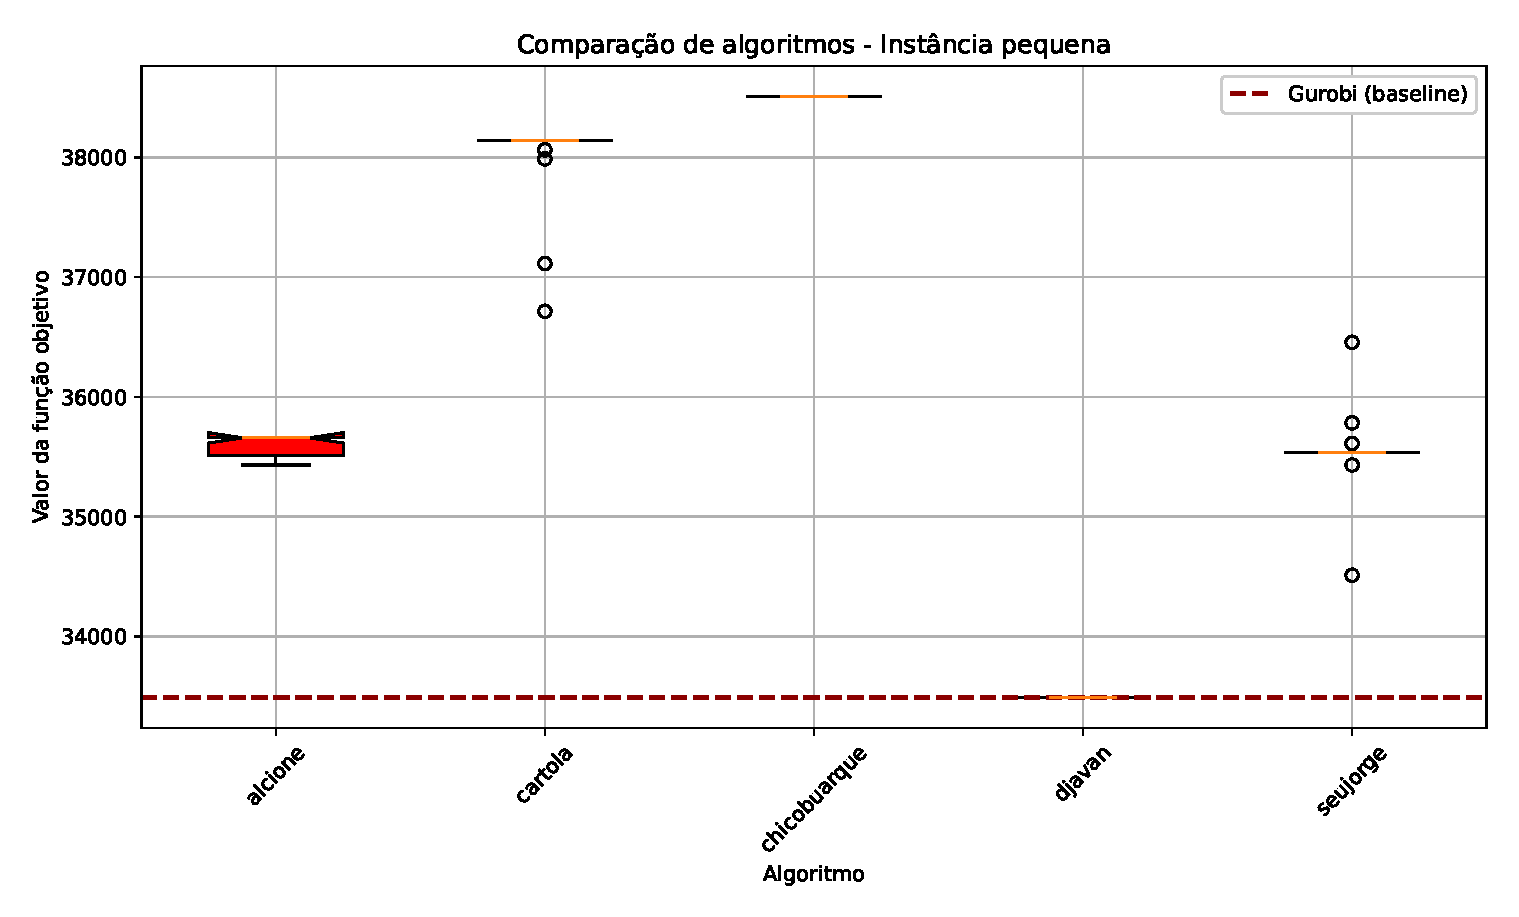
\includegraphics[width=0.8\textwidth]{boxplot_pequena.eps}
    \caption{Boxplot dos resultados para a instância pequena.}
\end{figure}
\end{frame}

\section{Instância Média}
\begin{frame}
\frametitle{Resultados}
\framesubtitle{Instância Média}
\begin{figure}
    \centering
    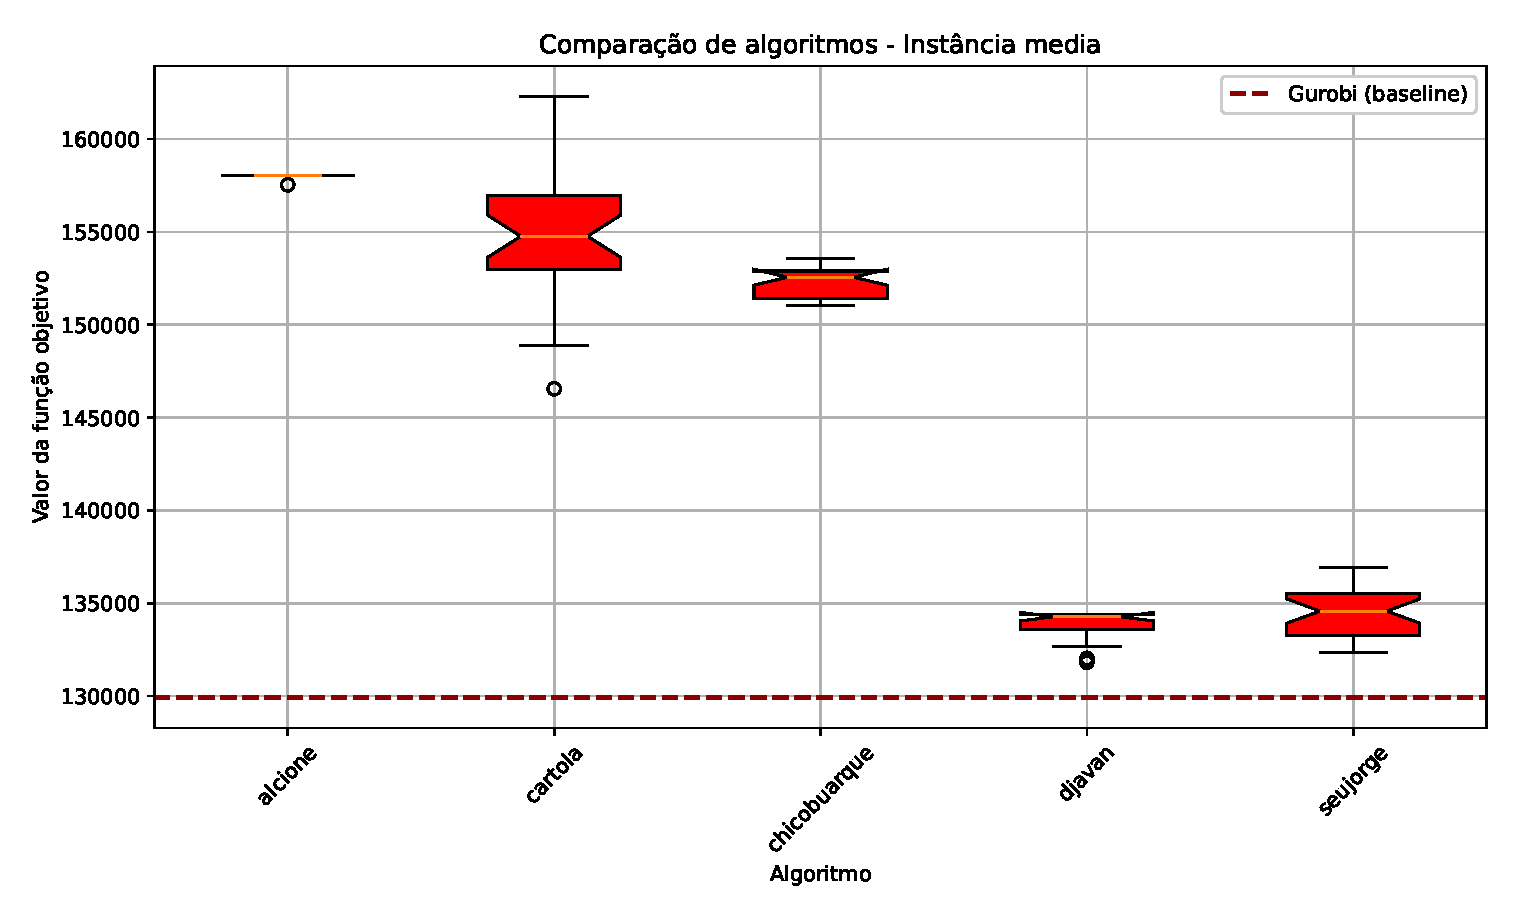
\includegraphics[width=0.8\textwidth]{boxplot_media.eps}
    \caption{Boxplot dos resultados para a instância média.}
\end{figure}
\end{frame}

\begin{frame}
\frametitle{Resultados}
\framesubtitle{Instância Média - Teste Estatístico}
\begin{itemize}
    \item Para verificar se há evidência estatística suficiente para afirmar qual algoritmo foi melhor: Djavan ou Seu Jorge.
    \item A distribuição dos dados do Djavan não foi aproximadamente normal (p-valor $< 0.05$ no teste de Shapiro-Wilk). Logo, foi utilizado o teste de Mann-Whitney U.
    \item P-valor obtido: 0.0975
    \item Não há evidência estatística suficiente para afirmar que um algoritmo foi melhor que o outro nesta instância com um nível de significância de 5\%.
\end{itemize}
\end{frame}

\section{Instância Grande}
\begin{frame}
\frametitle{Resultados}
\framesubtitle{Instância Grande}
\begin{itemize}
    \item Apenas 1 execução do Djavan resultou em solução não factível.
\end{itemize}
\begin{figure}
    \centering
    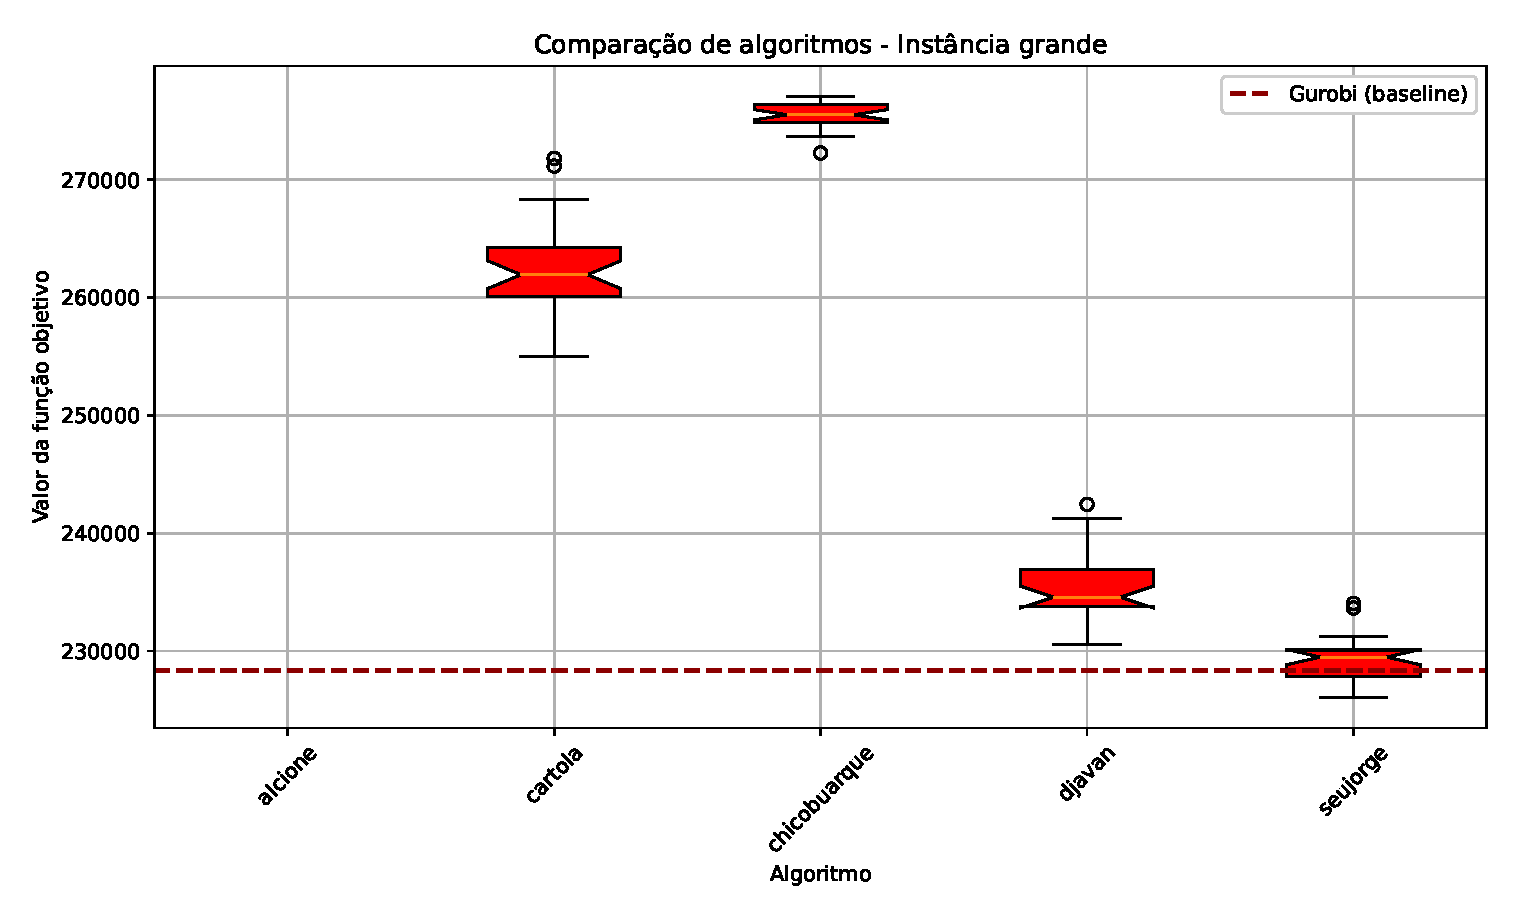
\includegraphics[width=0.8\textwidth]{boxplot_grande.eps}
    \caption{Boxplot dos resultados para a instância grande.}
\end{figure}
\end{frame}

\begin{frame}
\frametitle{Resultados}
\framesubtitle{Instância Grande - Teste Estatístico}
\begin{itemize}
    \item Para verificar se há evidência estatística suficiente para afirmar qual algoritmo foi melhor: Djavan ou Seu Jorge.
    \item Ambas distribuições são aproximadamente normais (p-valor $> 0.05$ no teste de Shapiro-Wilk). Logo, foi utilizado o teste t de Student com variâncias desiguais (Welch's t-test).
    \item P-valor obtido para a alternativa Dvajan $>$ Seu Jorge: $> 10^{-11}$.
    \item Há evidência estatística suficiente para afirmar que o algoritmo Djavan foi melhor que o Seu Jorge nesta instância com um nível de significância de 5\%.
\end{itemize}
\end{frame}

\section{Instância Rush}
\begin{frame}
\frametitle{Resultados}
\framesubtitle{Instância Rush}
\begin{itemize}
    \item 18 soluções factíveis para o Chico Buarque.
\end{itemize}
\begin{figure}
    \centering
    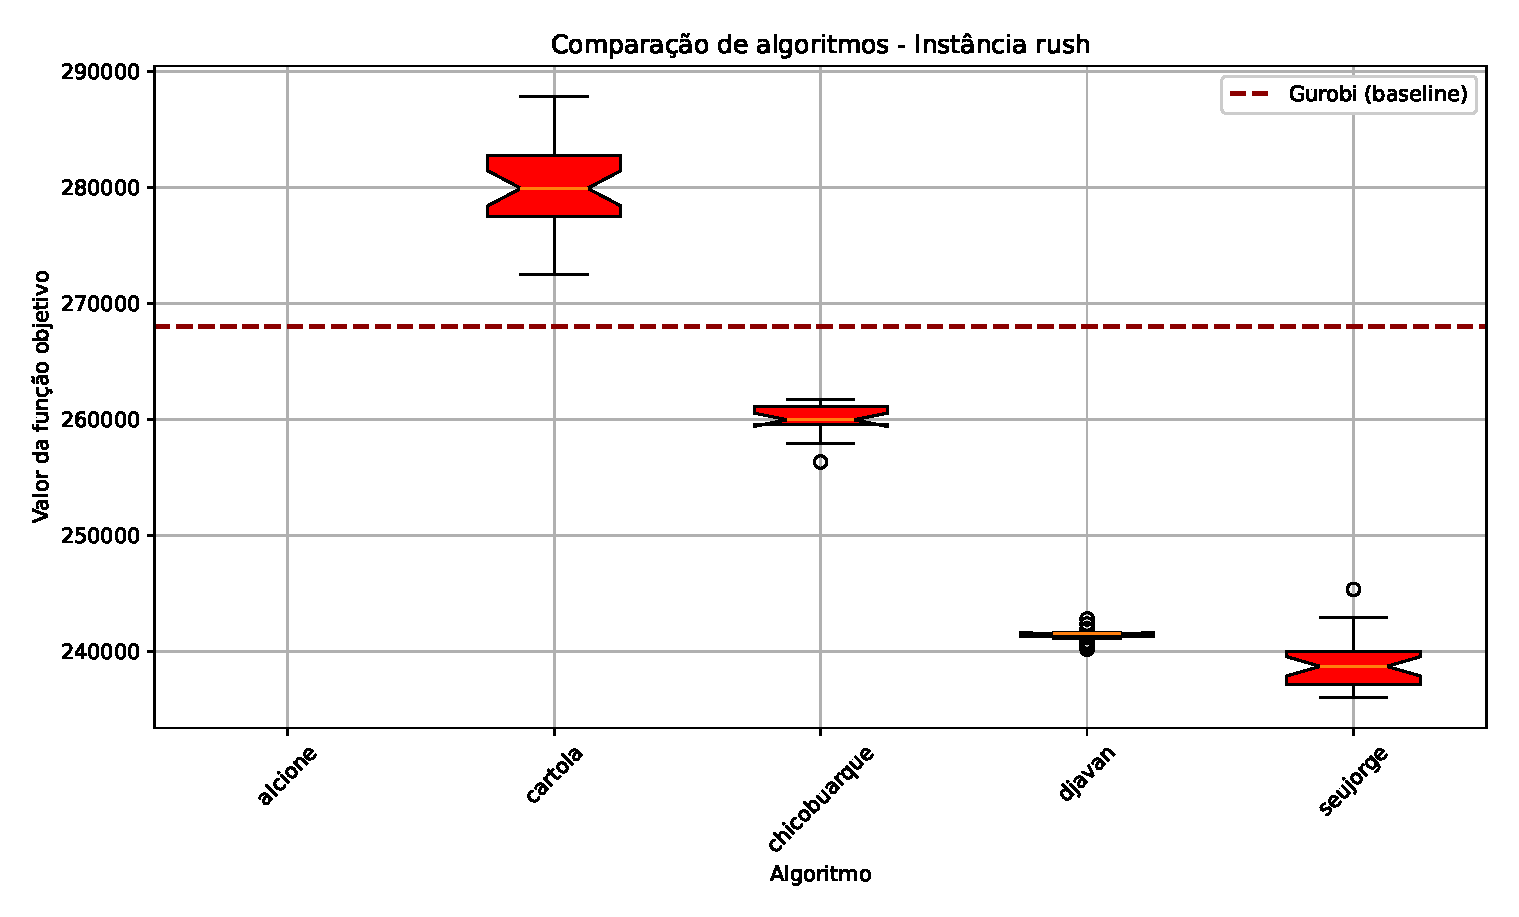
\includegraphics[width=0.8\textwidth]{boxplot_rush.eps}
    \caption{Boxplot dos resultados para a instância rush.}
\end{figure}
\end{frame}

\begin{frame}
\frametitle{Resultados}
\framesubtitle{Instância Rush - Teste Estatístico}
\begin{itemize}
    \item Para verificar se há evidência estatística suficiente para afirmar qual algoritmo foi melhor: Djavan ou Seu Jorge.
    \item A distribuição dos dados de ambos não foi aproximadamente normal (p-valor $< 0.05$ no teste de Shapiro-Wilk). Logo, foi utilizado o teste de Mann-Whitney U.
    \item P-valor obtido para a alternativa Dvajan $>$ Seu Jorge: $> 10^{-6}$.
    \item Há evidência estatística suficiente para afirmar que o algoritmo Djavan foi melhor que o Seu Jorge nesta instância com um nível de significância de 5\%.
\end{itemize}
\end{frame}

\end{document}